\section{Flyback converter}

The flyback converter is another option for a DC-DC converter. It has galvanic isolation between the input and the outputs. The flyback converter is basically a buck-boost converter, but here the inductor is split to form a transformer. The windings of the transformer can have different turns ratio and in that way it is possible to step the voltage and current both up or down \cite{flyback}. 

The basic circuit of the Flyback topology can be seen in figure \ref{Flyback_SCHEMATIC}. It consists of a DC-source, two switches (a transistor and a diode), two capacitors, a transformer and a load.    

\begin{figure}[H]
	\begin{center}
	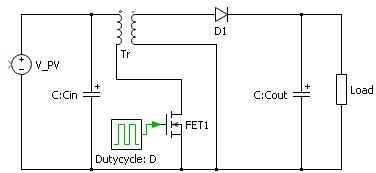
\includegraphics[width=0.7\textwidth]{../Pictures/flyback_schem.png}
	\caption{Flyback converter}
	\label{Flyback_SCHEMATIC}
	\end{center}
\end{figure}

When the MOSFET is on, the energy is transferred from the input voltage source to the transformer. In this state the output capacitor will supply the load with the output voltage. In the off-state the transformer will supply the output load with energy while it also charges the capacitor\cite{flyback}. 
The transformer makes it possible to have multiple secondary windings, and therefore different output voltages. This can be used when designing the supply voltage for the control system\cite{flyback}.

The transformer makes it possible to have multiple secondary windings, and therefore output voltages. This can be used when designing the supply voltage for the control system\cite{flyback}.  

The drawbacks are primarily the current and voltage waveforms. The voltage-drop across the two switches in their respective off periods, is decided by the input- and output voltages and the transfer ratio of the transformer. Furthermore the leakage inductance from the transformer will result in a big voltage spike at the rising edge of the drain source voltage ($V_{ds}$) of the MOSFET. These needs to be reduced by a snubber circuit, like a RCD-circuit placed in parallel with the MOSFET\cite{flyback}. This will increase the power loss and therefore decreasing the efficiency. The leakage inductance will also produce transients which will make the voltage stress at the MOSFET bigger and give high-frequency ringing at the input\cite{underthehood}. The $V_{ds}$ is showed at figure \ref{Flyback_waveforms} as $V_{SW}$.

%Because of the single control device another advantage of the flyback converter is a wide choice of controllers. For example, it is possible to directly connect a PWM IC to control the MOSFET, and thus, the converter. 

Even though the transformer is be driven in continuous conduction mode (CCM), the currents in the windings will be discontinuous. This means that the RMS currents in both the primary and the secondary windings becomes higher\cite{flyback}. The primary and secondary currents are shown at figure \ref{Flyback_waveforms} as $i_{pri}$ and $i_{sec}$ respectively.

\begin{figure}[H]
	\begin{center}
		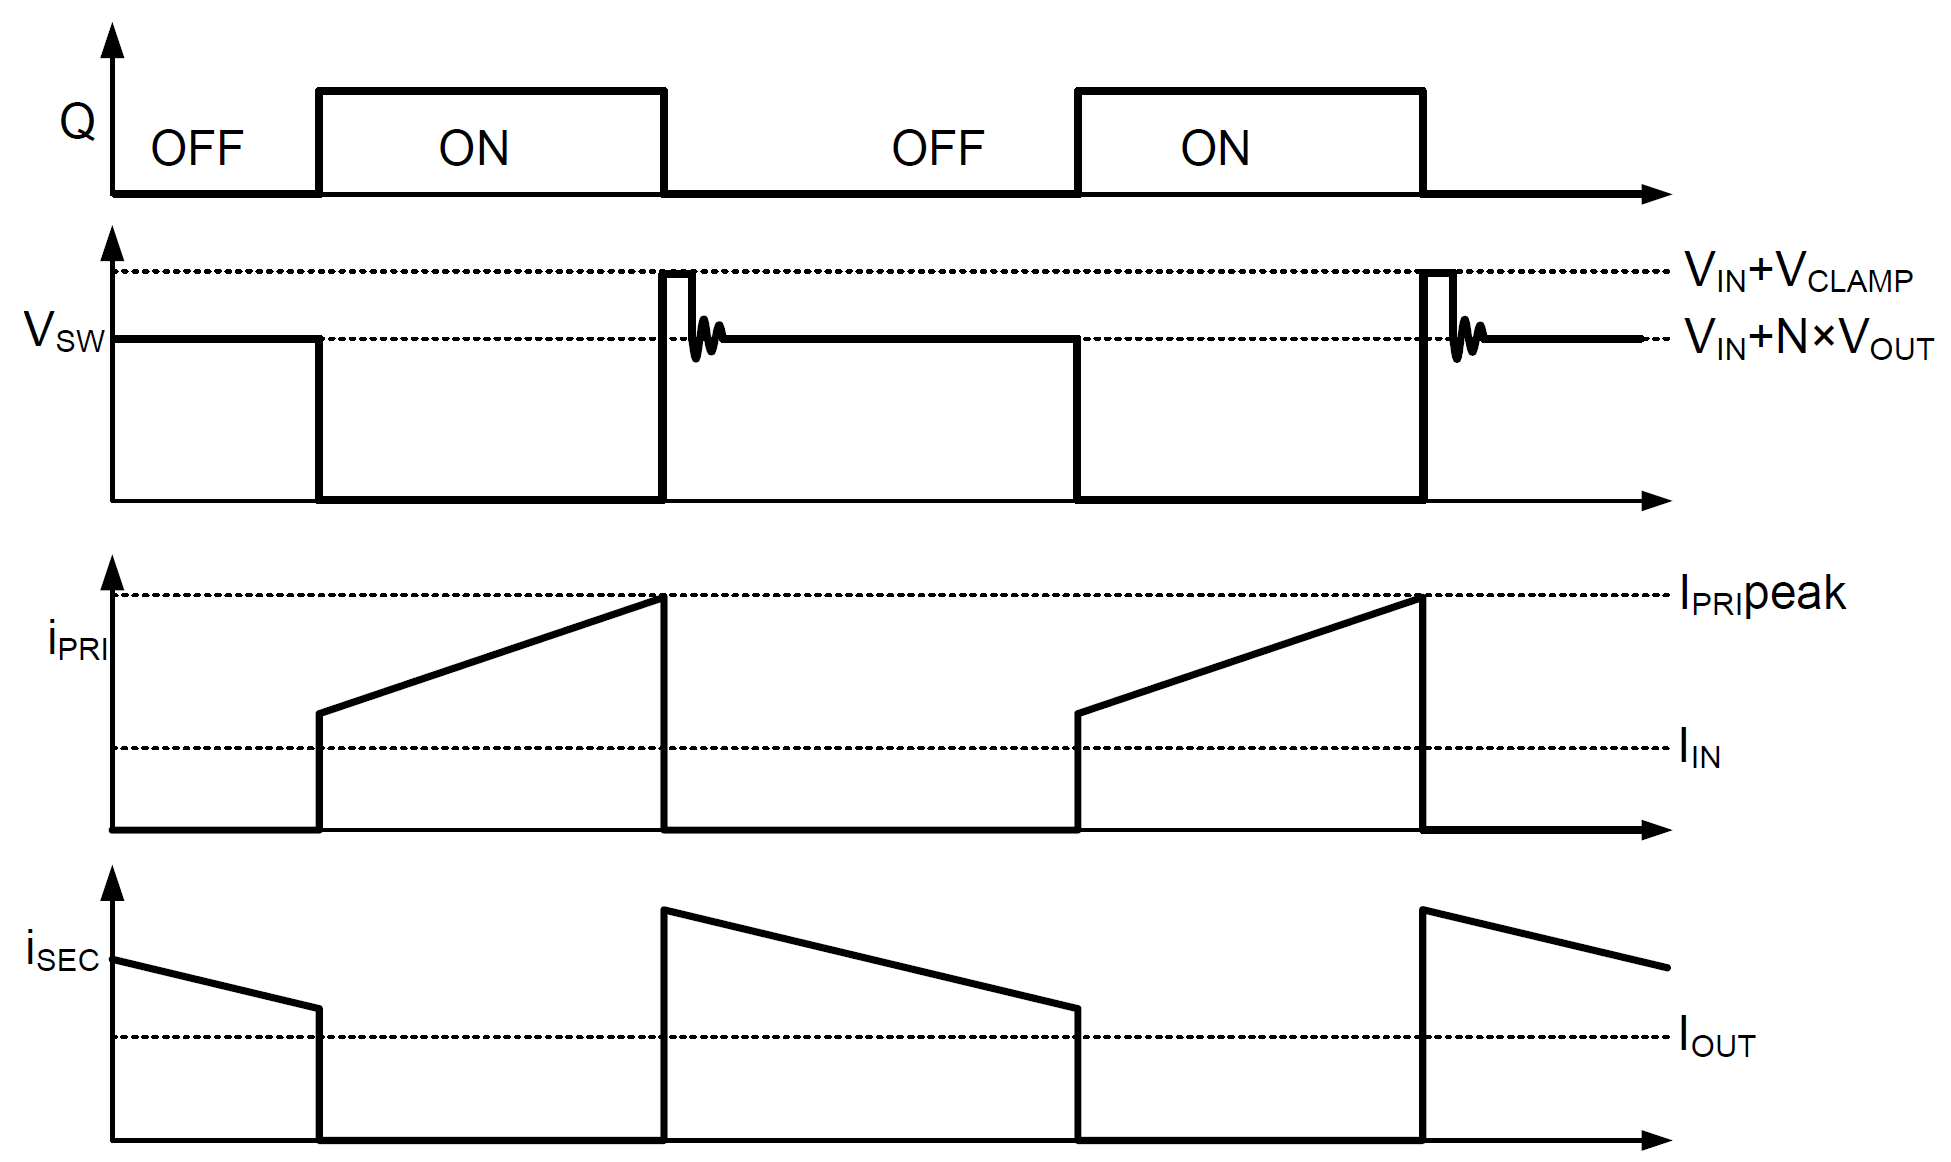
\includegraphics[width=0.7\textwidth]{../Pictures/flyback_waveforms.png}
		\caption{Flyback voltage and current waveforms\cite{flyback_waveforms}}
		\label{Flyback_waveforms}
	\end{center}
\end{figure}
